\ifdefined\COMPLETE
\else
    \input{./preambule-sacha-utf8.ltx}
    \begin{document}
\fi



\section{Lois à densité sur un intervalle}

\subsection{Variable aléatoire discrète, variable aléatoire continue}

\subsubsection{Rappel : Variable aléatoire discrète}

Soit $\Omega$ un espace probabilité fini. \\
Soit $X$ une variable aléatoire définie sur $\Omega$ ne prenant qu'un nombre fini de valeurs. \\

La \underline{loi de probabilité} $X$ est en général présentée sous fome d'un tableau. \\

\textbf{Exemple} : \\

\begin{tabular}{|c|c|c|c|c|}
\hline
$x$ & $x_1$ & $x_2$ & $x_3$ & $x_4$ \\
\hline
$p\left(x=x_i\right)$ & $0,4$ & $0,2$ & $0,3$ & $0,4$ \\
\hline 
\end{tabular}

\vspace*{.7cm}

On a $X\left(\Omega\right) = \lb x_1 \; ; \; x_2 \; ; \; x_3 \; ; \; x_4 \rb$. \\

De plus, on a bien $\somme{}{}{p\left(x=x_i\right)} = 1$. \\

On définit alors une fonction $f$ par $f(x) = p\left(X=x\right)$.

\subsubsection{Variable aléatoire continue}

Soit $\Omega$ un espace probabilisé fini. \\
Soit $X$ une variable aléatoire définie sur $\Omega$ qui peut prendre comme valeurs (au moins théoriquement) tous les nombres réels d'un intervalles $\left[a \; ; \; b\right]$ inclus dans $\R$. \\

Pour la loi de probabilité de $X$, on a recours à une fonction, appelée \underline{fonction de densité}, ou plus simplement \underline{densité}.

\subsection{Fonction de densité}

\subsubsection{Définition}

Soit $\left[a \; ; \; b\right]$ in intervalle inclus dans $\R$. \\

On appelle fonction de densité sur $\left[a \; ; \; b\right]$ toute fonction continue et positive sur $\left[a \; ; \; b\right]$ \\ et telle que $\displaystyle{ \int_a^b f(x) \; \diff x} = 1$.

\newpage

\subsubsection{Loi de probabilité d'une variable aléatoire continue munie d'une fonction de densité}

Soit $\Omega$ un espace probabilisé fini. \\
Soit $X$ une variable aléatoire continue de valeurs dans un intervalle $\left[a \; ; \; b\right]$ inclus dans $\R$. \\
Soit $f$ sa fonction de densité. \\

\begin{itemize}
\item[•] Probabilité d'un événement : \\

$p\left(a \leqslant X \leqslant b\right) = \displaystyle{\int_a^b f(x) \; \diff x} = 1$ \\

\begin{tikzpicture}[line cap=round,line join=round,>=triangle 45,x=2cm,y=1cm,scale=1]
\draw[->] (-0.5,0) -- (2.5,0);
% \foreach \x in {1}
% \draw[shift={(\x,0)}] (0pt,2pt) -- (0pt,-2pt) ; % node[below] {\footnotesize $\x$};
\draw (.5,0) node[below] {\footnotesize $a$}; % \draw (.5,3.2) node[above] {\footnotesize $x=a$}; 
\draw (2,0) node[below] {\footnotesize $b$}; % \draw (2,3.2) node[above] {\footnotesize $x=b$}; 

\draw[->] (0,-1.5) -- (0,3.5);
% \foreach \y in {1}
% \draw[shift={(0,\y)}] (2pt,0pt) -- (-2pt,0pt);  % node[left] {\footnotesize $\y$};
\draw (0pt,-8pt) node[left] {\footnotesize $0$};
% \draw (0,.5) node[left] {\footnotesize $\vec{i}$};
% \draw (0,1) node[left] {\footnotesize $B$};

\draw (1.25,0) node[below] {\footnotesize aire}; 
\draw (2,2.1) node[right] {\footnotesize $\mathcal{C}_f$}; 

\clip (0.5,-1) rectangle (2.01,4);



% \draw[pattern=north east lines, pattern color=blue] (0,0) rectangle (1,1) ; 
\draw [fill=white] (0,0) rectangle (.125,.25) ; 

\draw (2,2.2) node[right] {\footnotesize $\mathcal{C}_f $};

\draw [smooth, samples=100,domain=0.2:2.5]  plot(\x,{(26/15)*(\x)^3 -(31/5)*(\x)^2 +(20/3)*(\x) -(1/5)}) ; 

\fill [pattern=north east lines, smooth, samples=100,domain=0.5:2] (0.5,0) -- (.5, 1.8) -- plot(\x,{(26/15)*(\x)^3 -(31/5)*(\x)^2 +(20/3)*(\x) -(1/5)}) -- (2,2.2) -- (2,0) -- cycle ;

\draw(.5,0) -- (.5,1.8) ; 
\draw(2,0) -- (2,2.2) ; 



\begin{pgfonlayer}{background}   
\draw[step=1mm,ultra thin,AntiqueWhite!10] (-0.5,-1) grid (2.6,4);
\draw[step=5mm,very thin,AntiqueWhite!30] (-0.5,-1) grid (2.6,4);
\draw[step=1cm,very thin,AntiqueWhite!50]  (-0.5,-1) grid (2.6,4);
\draw[step=5cm,thin,AntiqueWhite]           (-0.5,-1) grid (2.6,4);
\end{pgfonlayer}

\end{tikzpicture}

\vspace*{.3cm}

\item[•] Soient $c \in \left[a \; ; \; b\right)$ et $d \in \left[a \; ; \; b\right)$, avec $c < d$. \\
$p\left(c \leqslant X \leqslant d\right) = \displaystyle{\int_c^d f(x) \; \diff x}$. \\

\begin{tikzpicture}[line cap=round,line join=round,>=triangle 45,x=2cm,y=1cm,scale=1]
\draw[->] (-0.5,0) -- (2.5,0);

\draw (.5,0) node[below] {\footnotesize $a$}; % \draw (.5,3.2) node[above] {\footnotesize $x=a$}; 
\draw (2,0) node[below] {\footnotesize $b$}; % \draw (2,3.2) node[above] {\footnotesize $x=b$}; 

\draw[->] (0,-1.5) -- (0,3.5);

\draw (0pt,-8pt) node[left] {\footnotesize $0$};


\draw (1.25,0) node[below] {\footnotesize aire}; 
\draw (2,2.1) node[right] {\footnotesize $\mathcal{C}_f$}; 

\clip (0.49,-1) rectangle (2.01,4);

\draw [fill=white] (0,0) rectangle (.125,.25) ; 

\draw (2,2.2) node[right] {\footnotesize $\mathcal{C}_f $};

\draw [smooth, samples=100,domain=0.2:2.5]  plot(\x,{(26/15)*(\x)^3 -(31/5)*(\x)^2 +(20/3)*(\x) -(1/5)}) ; 

\fill [pattern=north east lines, smooth, samples=100,domain=0.75:1.75] (0.75,0) -- (.75, 1.8) -- plot(\x,{(26/15)*(\x)^3 -(31/5)*(\x)^2 +(20/3)*(\x) -(1/5)}) -- (1.75,0) -- cycle ;

\draw (.5,0) -- (.5,1.8) ; 
\draw(2,0) -- (2,2.2) ; 

\draw  (.75,0) node [below] {\footnotesize $c$} -- (.75,2) ; 
\draw  (1.75,0) node [below] {\footnotesize $d$}  -- (1.75,1.75) ; 


\begin{pgfonlayer}{background}   
\draw[step=1mm,ultra thin,AntiqueWhite!10] (-0.5,-1) grid (2.6,4);
\draw[step=5mm,very thin,AntiqueWhite!30] (-0.5,-1) grid (2.6,4);
\draw[step=1cm,very thin,AntiqueWhite!50]  (-0.5,-1) grid (2.6,4);
\draw[step=5cm,thin,AntiqueWhite]           (-0.5,-1) grid (2.6,4);
\end{pgfonlayer}

\end{tikzpicture}
\end{itemize}

\vspace*{.3cm}

\textbf{En conséquence :} On a $p\left(X = c\right) = 0$. \\

Donc $p\left(c < X \leqslant d\right) = p\left(c \leqslant X < d\right) = p\left(c < X < d\right)$. \\

Ainsi, l'utilisation d'intervalles ouvertes ou fermés n'a pas d'importance. \\

\textbf{Remarque :} Les propriétés des probabilités dans le cas discret détendent au cas continu. 

\newpage

\vspace*{-2cm}

\subsubsection{Exemples}

\textbf{Exemple n°1} 

Soit f la fonction définie sur $\left[a \; ; \; b\right]$ par : \\

\begin{tikzpicture}[line cap=round,line join=round,>=triangle 45,x=1.0cm,y=10cm]
\draw[->] (-0.63,0) -- (4.5,0);
\foreach \x in {1,2,3,4}
\draw[shift={(\x,0)}] (0pt,2pt) -- (0pt,-2pt) node[below] {\footnotesize $\x$};
\draw[->] (0,-0.05) -- (0,.6);
\foreach \y in {0.1,0.2,0.3,0.4,0.5}
\draw[shift={(0,\y)}] (2pt,0pt) -- (-2pt,0pt) node[left] {\footnotesize $\y$};
\draw (0pt,-10pt) node[right] {\footnotesize $0$};
\clip (-0.63,-0.05) rectangle (5.5,0.65) ;

\fill [pattern color=DarkGreen, pattern=north east lines] (0,0) -- (1,.4) -- (2,0) -- (4,0.1) -- (4,0)  -- cycle ;

\draw [color=blue] (0,0)-- ++(-1.5pt,-1.5pt) -- ++(3.0pt,3.0pt) ++(-3.0pt,0) -- ++(3.0pt,-3.0pt);
\draw [color=blue] (1,.4)-- ++(-1.5pt,-1.5pt) -- ++(3.0pt,3.0pt) ++(-3.0pt,0) -- ++(3.0pt,-3.0pt);
\draw [color=blue] (2,0)-- ++(-1.5pt,-1.5pt) -- ++(3.0pt,3.0pt) ++(-3.0pt,0) -- ++(3.0pt,-3.0pt);
\draw [color=blue] (4,0.1)-- ++(-1.5pt,-1.5pt) -- ++(3.0pt,3.0pt) ++(-3.0pt,0) -- ++(3.0pt,-3.0pt);
\draw [blue] (0,0) -- (1,.4) -- (2,0) -- (4,0.1) ; 
\draw[dashed] (0,0.1) -- (4,0.1) -- (4,0) ; 

\begin{pgfonlayer}{background}   
\draw[step=1mm,ultra thin,AntiqueWhite!10] (-0.63,-0.05) grid (5,0.65) ;
\draw[step=5mm,very thin,AntiqueWhite!30]  (-0.63,-0.05) grid (5,0.65) ;
\draw[step=1cm,very thin,AntiqueWhite!50]  (-0.63,-0.05) grid (5,0.65) ;
\draw[step=5cm,thin,AntiqueWhite]          (-0.63,-0.05) grid (5,0.65) ;
\end{pgfonlayer}

\end{tikzpicture}

\vspace*{.3cm}

\textbf{Remarque :} On dit que $f$ est une \underline{fonction affine par morceaux}. \\

\begin{itemize}
\item[1.] Montrer que $f$ est une fonction de densité sur $\left[a \; ; \; b\right]$. \\

\begin{itemize}
\item[•] $f$ est définie, continue et positive sur $\left[a \; ; \; b\right]$. 
\item[•] $\displaystyle{\int_a^b f(x) \; \diff x} = \dfrac{1}{2} \times 2 \times 0,8 + \dfrac{1}{2} \times 2 \times 0,2 = 0,8 + 0,2 = 1$. L'aire de la portion hachurée est $1$. \\

Donc $f$ est bien une fonction de densité sur $\left[a \; ; \; b\right]$. \\
\end{itemize}

\item[2.] Soit \hbox{$X$ une variable aléatoire continue à valeurs sur $\left[0 \; ; \; 4\right]$, dont la loi de probabilité est la fonction $f$.} \\

\begin{itemize}
\item[•] Déterminer $p\left(1 \leqslant x \leqslant 2\right)$. \\

On a $p\left(1 \leqslant x \leqslant 2\right) = \displaystyle{\int_1^2 f(x) \; \diff x} = \dfrac{1}{2}\left(\dfrac{1}{2} \times 2 \times 0,8\right) = 0,4$

\vspace*{.3cm}

\item[•] Déterminer $p_{1 \leqslant x \leqslant 2}\left(1,5 \leqslant x \leqslant 2,5\right)$. \\

On a $p_{1 \leqslant x \leqslant 2}\left(1,5 \leqslant x \leqslant 2,5\right) = \dfrac{p\left[\left(1 \leqslant x \leqslant 2\right) \cap \left(1,5 \leqslant x \leqslant 2,5\right)\right]}{p\left(1 \leqslant x \leqslant 2\right)}$. \vspace*{.3cm} \\

\begin{tikzpicture}
     \tkzInit[xmin=0,xmax=3.5,xstep=.3] % Plus xstep est grand, 
                                                           % plus le dessin est sérré
     \tkzDrawX[label={},noticks,nograd]
      \tkzText(0,.5){0}
     \tkzText(1,.5){1}
     \tkzText(1.5,.5){1.5}
          \tkzText(2,.5){2}
     \tkzText(2.5,.5){2.5}
     
     \tkzXH[color=black]   
     {
        0/T//1.5/T/[,   
         2.5/T/]/3.4/T/       
     }     
     \tkzXHW[color=green]    
     {
      0/T//1/T/[,
        2/T/]/3.4/T/
     }
\end{tikzpicture}

\vspace*{.3cm}

Ainsi $p_{1 \leqslant x \leqslant 2}\left(1,5 \leqslant x \leqslant 2,5\right) = \dfrac{p\left(1,5 \leqslant x \leqslant 2\right)}{p\left(1 \leqslant x \leqslant 2\right)}$. \vspace*{.3cm} \\


Or, on a $p\left(1,5 \leqslant x \leqslant 2\right) = \displaystyle{\int_{1,5}^2 f(x) \; \diff x} = \dfrac{1}{2} \times 0,5 \times 0,4 = 0,1$. \\

\vspace*{.3cm}

Donc $p\left(1,5 \leqslant x \leqslant 2\right) = 0,1$. \\

Ainsi $p_{1 \leqslant x \leqslant 2}\left(1,5 \leqslant x \leqslant 2,5\right) = \dfrac{0,1}{0,4} = \dfrac{1}{4}$.

\end{itemize}
\end{itemize} 

\newpage

\textbf{Exemple n°2} \\

La production quotidienne $X$ d'une produit est une variable aléatoire continue à valeurs dans l'intervalle $\left[0 \; ; \; 10\right]$, qui a pour fonction de densité la fonction $f$ définie par $f(x) = 0,006\left(10x-x^2\right)$. $X$ est exprimé en tonnes. \\

\begin{itemize}
\item[1.] Vérifier que $f$ est bien une fonction de densité sur $\left[0 \; ; \; 10\right]$. \\ 

\begin{itemize}
\item[•] $f$ est une fonction polynôme du second degré. $f$ est donc définie et continue sur $\left[0 \; ; \; 10\right]$. \\

On a $f(x) = 0,006\left(10x-x^2\right) = -0,006x^2 + 0,06x$. \\

De plus, $f(x) = 0 \Longleftrightarrow x = 0$ ou $x = 10$. \\

On en déduit le tableau de signes suivant \\

\begin{tikzpicture}
\tkzTabInit[lgt=5,espcl=2]
{ $x$               /1,
$f(x)$    /1}
{$ - \infty $ , $0$, $10$, $+ \infty $}
\tkzTabLine{ , - , z , + , z , - , }
\end{tikzpicture}

\vspace*{.3cm}

$f$ est donc positif sur $\left[0 \; ; \; 10\right]$. \\

\item[•] On calcule $\displaystyle{\int_0^{10} f(x) \; \diff x}$. \\

On a $\displaystyle{\int_0^{10} f(x) \; \diff x} = F\left(10\right) - F\left(0\right)$. \\

On a $f(x) = -0,006x^2 + 0,006x$, donc $F(x) = -0,002x^3 + 0,03x^2$. \\

Ainsi $F(10) = 1$ et $F(0) = 0$. \\

Donc $\displaystyle{\int_0^{10} f(x) \; \diff x} = F\left(10\right) - F\left(0\right) = 1 - 0 = 1$. \\

Donc $f$ est bien une fonction de densité sur $\left[0 \; ; \; 10\right]$.
\end{itemize}

\vspace*{.3cm}

\item[2.] Déterminer $p\left(X \leqslant 7\right)$ et $p\left(X > 6\right)$. \\

\begin{itemize}
\item[•] $p\left(X \leqslant 7\right) = p\left(0 \leqslant X \leqslant 7\right) = \displaystyle{\int_0^7 f(x) \; \diff x} = F(7) - F(0) = 0,784 - 0 = 0,784$. \\

\vspace*{.3cm}

\item[•] $p\left(X > 6\right) = p\left(6 \leqslant X \leqslant 10\right) = \displaystyle{\int_6^{10} f(x) \; \diff x} = F(10) - F(6) = 1 - 0,648 = 0,352$.
\end{itemize}
\end{itemize}




\newpage

\subsection{Loi uniforme sur un intervalle $\left[a \; ; \; b\right]$}

\subsubsection{Définition}

Soit $X$ une fonction aléatoire \textbf{continue} sur un intervalle $\left[a \; ; \; b\right]$. \\
Soit $f$ une fonction de densité de la loi de probabilité $X$. \\

On dit que \underline{$X$ sur la loi uniforme sur $\left[a \; ; \; b\right]$} si et seulement si la fonction $f$ est une \underline{fonction constante} sur $\left[a \; ; \; b\right]$. \\

On a alors pour tout $x \in \left[a \; ; \; b\right], f(x) = \lambda$. \\

\begin{tikzpicture}[line cap=round,line join=round,>=triangle 45,x=1cm,y=1cm,scale=1]
\draw[->] (-0.5,0) -- (5,0);
 
\draw[->] (0,-.5) -- (0,4.5);

\draw (0pt,-8pt) node[left] {\footnotesize $0$};

\draw [dashed] (0,3.5) node [left] {\footnotesize $f(x)$} --  (1,3.5) -- (1,0) node[below] {\footnotesize $a$}; 
\draw  (1,3.5) -- (4,3.5) ;
\draw  [dashed] (4,3.5) -- (4,0) node[below] {\footnotesize $b$}; 

\begin{pgfonlayer}{background}   
\draw[step=1mm,ultra thin,AntiqueWhite!10] (-0.7,-1) grid (5,5.5) ;
\draw[step=5mm,very thin,AntiqueWhite!30]  (-0.7,-1) grid (5,5.5) ;
\draw[step=1cm,very thin,AntiqueWhite!50]  (-0.7,-1) grid (5,5.5) ;
\draw[step=5cm,thin,AntiqueWhite]          (-0.7,-1) grid (5,5.5) ;
\end{pgfonlayer}

\end{tikzpicture}

\vspace*{.3cm}

$f$ est une fonction constante sur $\left[a \; ; \; b\right]$, tel que $\forall x \in \R, f(x) = \lambda$. \\

On calcule $\displaystyle{\int_a^b f(x) \; \diff x} = \lambda$. \\

On sait que $\displaystyle{\int_a^b f(x) \; \diff x} = F(b) - F(a)$. \\

On a $f(x) = \lambda$, d'où $F(x) = \lambda x$. \\

Ainsi on a $F(b) = \lambda b$ et $F(a) = \lambda a$. \\

D'où $\displaystyle{\int_a^b f(x) \; \diff x} = \lambda b - \lambda a = \lambda\left(b-a\right)$. \\

Or, on sait que $\displaystyle{\int_a^b f(x) \; \diff x} = 1$. \\

Il vient que $\lambda\left(b-a\right) = 1$. \\

Donc $\lambda = \dfrac{1}{b-a}$. 

\newpage 

\subsubsection{Probabilité d'un événement}

Soit $X$ une variable aléatoire continue suivant la loi uniforme sur $\left[a \; ; \; b\right]$. \\
Soient $c \in \left[a \; ; \; b\right]$ et $d \in \left[ a\; ; \; b\right]$, avec $c < d$. \\

On cherche à déterminer $p\left(c \leqslant x \leqslant d\right)$. \\

On a $p\left(c \leqslant x \leqslant d\right) = \displaystyle{\int_c^d f(x) \; \diff x} = F(d) - F(c)$. \\

On a $f(x) = \dfrac{1}{b-a}$. \\

Donc $F(x) = \dfrac{1}{b-a}x$. \\

Ainsi $F(d) = \dfrac{1}{b-a}d$ et $F(c) = \dfrac{1}{b-a}c$. \\

On en conclut que $\displaystyle{\int_c^d f(x) \; \diff x} = \left(\dfrac{1}{b-a}d\right)-\left(\dfrac{1}{b-a}c\right) = \dfrac{d-c}{b-a}$. \\

Ainsi pour tout $c \in \left[a \; ; \; b\right]$, pour tout $d\left[a \; ; \; b\right]$, tels que $c < d$, $p\left(c \leqslant x \leqslant d\right) = \dfrac{d-c}{b-a}$.

\subsubsection{Espérance mathématique}

Soit $X$ une variable aléatoire continue suivant la loi uniforme sur $\left[a \; ; \; b\right]$. \\

\textbf{Rappel :} Si $X$ est une variable aléatoire discrète, on a $E(x) = \somme{}{}{x_ip\left(X=x_i\right)}$ et $f\left(x_i\right) = p\left(X=x_i\right)$. \\

On a ici $E\left(x\right) = \displaystyle{\int_a^b xf(x) \; \diff x} = \displaystyle{\int_a^b x\dfrac{1}{b-a} \; \diff x} = \dfrac{1}{b-a}\displaystyle{\int_a^b x \; \diff x}$. \\

On pose $g(x) = x$. \\

On a alors $G(x) = \dfrac{1}{2}x^2$. \\

Donc $G\left(b\right) = \dfrac{1}{2}b^2$ et $G\left(a\right) = \dfrac{1}{2}a^2$. \\

Ainsi $\displaystyle{\int_a^b g(x) \; \diff x} = \dfrac{1}{2}b^2 - \dfrac{1}{2}a^2 = \dfrac{b^2 - a^2}{2}$. \\

\vspace*{.3cm}

\begin{tabular}{lll}
\hspace{-.3cm} D'où $E\left(X\right)$ & $=$ & $\dfrac{1}{b-a} \times \dfrac{b^2 - a^2}{2}$ \vspace*{.3cm} \\
& $=$ & $\dfrac{1}{b-a} \times \dfrac{\left(b-a\right)\left(b+a\right)}{2}$ \vspace*{.3cm} \\
& $=$ & $\dfrac{b+a}{2}$ \vspace*{.3cm} \\
& $=$ & $\dfrac{a+b}{2}$ \\
\end{tabular}

\vspace*{.3cm}

Ainsi, on a $E\left(X\right) = \dfrac{a+b}{2}$.

\newpage

\vspace*{-2cm}

\subsubsection{Exemples}

\textbf{Exemple n°1} 

Sylvain dit à Sylvette qu'il passera la voir entre 18h30 et 20h45. \\
Sylvette prend sa douche entre 19h et 19h30. \\

Quelle est la probabilité que Sylvain arrive alors que Sylvette est en train de prendre sa douche ? \\

Par convention, choisir un nombre au hasard dans un intervalle $\left[a \; ; \; b\right]$, c'est le choisir selon la loi uniforme sur $\left[a \; ; \; b\right]$. \\

Soit $X$ la variable aléatoire continue correspondant à l'heure d'arrivée de Sylvain. \\
$X$ prend ses valeurs dans $\left[18,5 \; ; \; 20,75\right]$. \\
$X$ suit la loi uniforme sur $\left[18,5 \; ; \; 20,75\right]$. \\

On cherche $p\left(19 \leqslant X \leqslant 19,5\right)$. \\

$p\left(19 \leqslant X \leqslant 19,5\right) = \dfrac{19,5-19}{20,75-18,5} = \dfrac{0,5}{2,25} = \dfrac{2}{9}$. \\

Il y a donc 2 chances sur 9 pour que Sylvain arrive au moment opportun. \\

\textbf{Exemple n°2} 

Une enquête a révélé que pour tout le personnel d'une grosse entreprise, le trajet entre domicile et lieu de travail est compris entre 0h30 et 2h30. \\

Soit $X$ la variable aléatoire continue correspondante à la durée du trajet d'un salarié. \\

\begin{itemize}
\item[1.] Quelle est la loi suivie par $X$ ? Déterminer et représenter sa fonction de densité. \\

\begin{tabular}{ll}
\begin{minipage}{8.5cm}
$X$ est une variable aléatoire continue sur $\left[0,5 \; ; \; 2,5\right]$. \\
$X$ suit la loi uniforme sur $\left[0,5 \; ; \; 2,5\right]$. \\

Soit $f$ la fonction de densité de la loi de probabilité de $X$. \\

Pour tout $x \in \left[0,5 \; ; \; 2,5\right], f(x) = \dfrac{1}{b-a} = \dfrac{1}{2,5-0,5} = \dfrac{1}{2}$. \\

\item[2.] Quelle est la probabilité que la durée du trajet d'un employé soit inférieure à 1h15 ? \\
\end{minipage}
&
\begin{minipage}{10cm}
\begin{tikzpicture}[line cap=round,line join=round,>=triangle 45,x=2cm,y=2cm,scale=1]
\draw[->] (-.25,0) -- (3.5,0);
\foreach \x in {1,2,3}
\draw[shift={(\x,0)}] (0pt,2pt) -- (0pt,-2pt) node[below] {\footnotesize $\x$};
\draw[->] (0,-.25) -- (0,2);
\foreach \y in {0.25,1,1.5}
\draw[shift={(0,\y)}] (2pt,0pt) -- (-2pt,0pt) node[left] {\footnotesize $\y$};
\draw (0pt,-5pt) node[left] {\footnotesize $0$};

\draw [pattern=north east lines] (.5,0) rectangle (2.5,0.5) ;  

\begin{pgfonlayer}{background}   
\draw[step=1mm,ultra thin,AntiqueWhite!10] (-.3,-.3) grid (3.7,2.2) ;
\draw[step=5mm,very thin,AntiqueWhite!30]  (-.3,-.3) grid (3.7,2.2) ;
\draw[step=1cm,very thin,AntiqueWhite!50]  (-.3,-.3) grid (3.7,2.2) ;
\draw[step=5cm,thin,AntiqueWhite]          (-.3,-.3) grid (3.7,2.2) ;
\end{pgfonlayer}

\end{tikzpicture}
\end{minipage}
\\
\end{tabular}

$\; \; $ On cherche $p\left(0,5 \leqslant X \leqslant 1,25\right)$.  \\

$\; \; $ On a $p\left(0,5 \leqslant X \leqslant 1,25\right) = \dfrac{1,25-0,5}{2,5-0,5} = \dfrac{0,45}{2} = \dfrac{3}{8}$. \\

$\; \; $ Il y a 3 chances sur 8 que le trajet domicile / entreprise dure moins de 1h25. \\

\item[3.] Quelle est la durée moyenne du trajet domicile / entreprise ? \\

$\; \;$ On sait que $E\left(X\right) = \dfrac{a+b}{2}$. \\

$\; \; $ Ici, $E\left(X\right) = \dfrac{0,5 + 2,5}{2} = \dfrac{3}{2}$. \\

$\; \; $ La durée moyenne est donc de 1h30.

\vspace*{-5cm}

\end{itemize}

\vspace*{-5cm}


\ifdefined\COMPLETE
\else
    \end{document}
\fi